\documentclass[12pt]{article}
\usepackage{cite}
\usepackage{url}
\usepackage{graphicx}

\title{Harvest \\
\large subtrop: SA Subtropical Harvest Growers' Association
}
\author{Binary Ninjaz \and Letanyan Arumugam \and Sizo Duma \and John Ojo \and Kevin Reid \and Shaun Yates \and Teboho}

\date{}

\renewcommand{\and}{\\}

\begin{document}
	\maketitle
	\begin{center}
	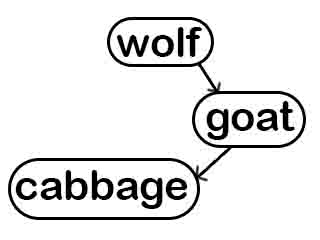
\includegraphics{team}	
	\end{center}
	
    \pagenumbering{gobble}
    \pagenumbering{arabic}

	\newpage
	
	\section*{Description}
	We envision using the mobile phones that the worker uses as simply a tracking device. They will not have to use it much other than start a timer when they start working and stop it once their done. Their GPS location will be polled periodically. The final yield amount will then be entered at the end. The rest of the predictive analysis and summary data will then be appropriately calculated. The summary and predications can then be accessed on a summary screen. The summary screen can be displayed on the mobile application and on the web interface. The web interface will be larger more customizable interface that will allow the farmers to do all maintenance and administrative work. The farmers will then have full access to summaries, projection trends and real-time locations.
	
	The following diagram shows how we intend to structure the entire system. We also show what the main functions that each view have to fulfil their desired design goals.
	
	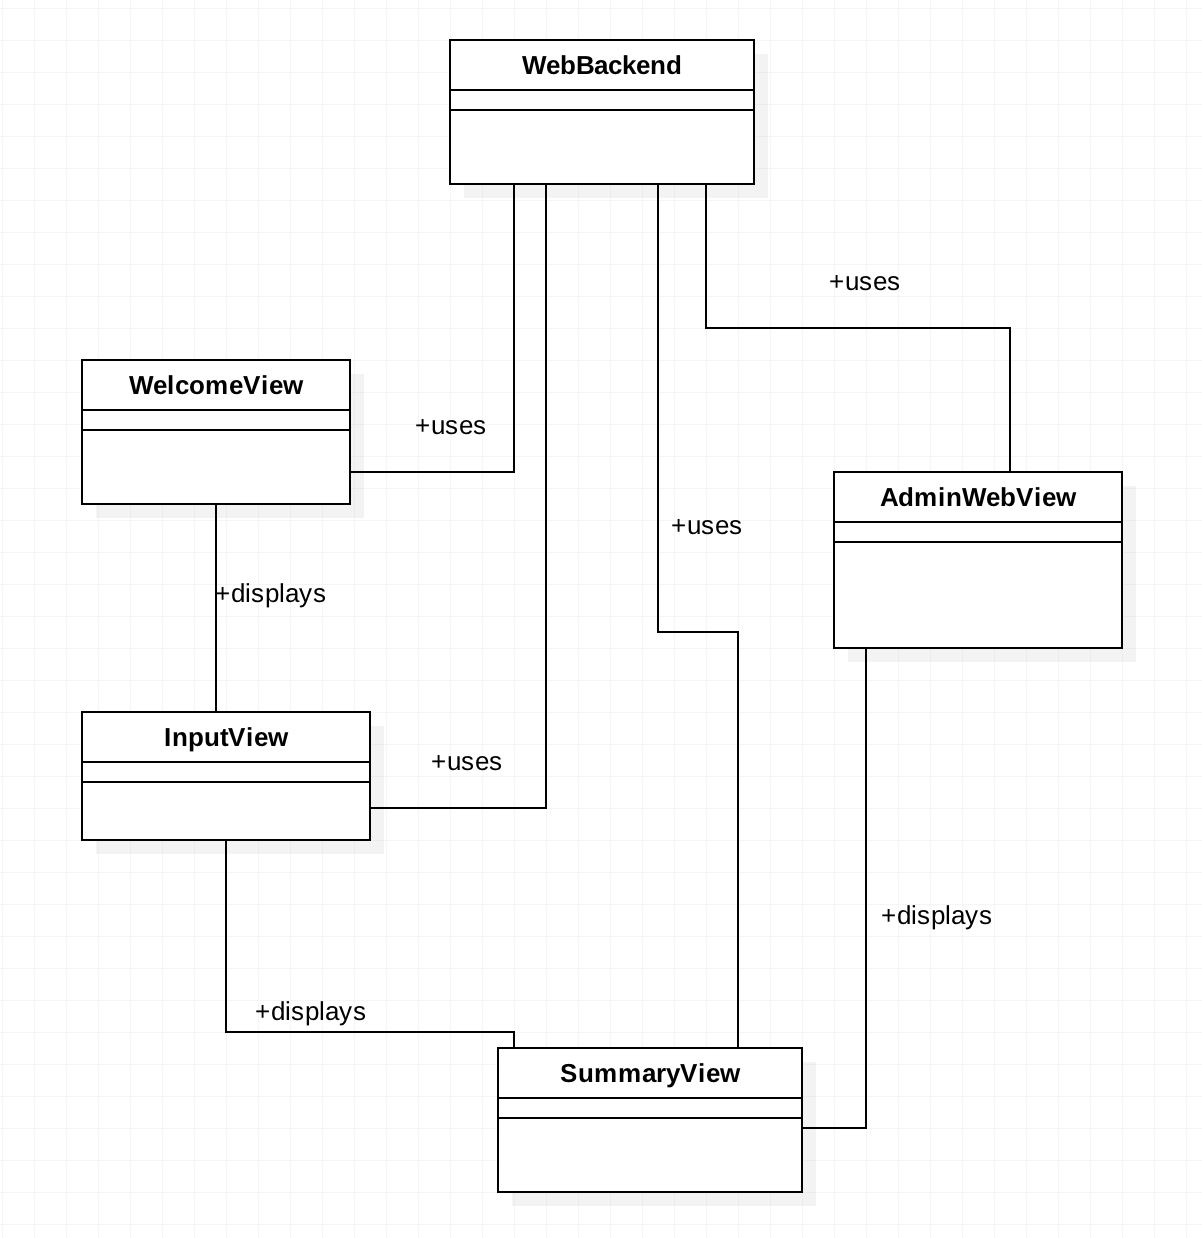
\includegraphics[scale=0.45]{Harvest.png}
	\newpage
	
	\section*{Technologies We'll Use}
	\begin{enumerate}
	\item Languages: HTML / CSS / JavaScript / Java / Swift
	\item Geographic Data: Google Maps API
	\item IDE: Android Studio / XCode
	\item Version Control: Git/Github
	\end{enumerate}
	
	\section*{Development Methodology}
	We are a diverse group of students from studies that all have a different focus. We intend to combine all of our own unique development strategies in-order to build the best and most understood application possible. We believe that everything can be made easier. And we enjoying making it so! We see your problem as being perfectly catered towards having an elegant solution. Data capturing user interfaces we one of the very first problems people needed to solve, which means we have a lot of history and design principles to guide us towards an optimal solution. The hardest part of creating a great data capturing user experience is understanding the work flow of the capturers. To accomplish this we will require interviews with the participants using the application and interface. We believe this will allow us a true understanding, which will allow us to build the perfect system.
	
	\section*{Who We Are}
	\subsection*{Letanyan Arumugam}
I am currently a 3rd-year student at the University of Pretoria studying BSc. Computer Science. In my spare time, I'm an
active member of the Swift-Evolution community, which deals with the language design of, the programming language, Swift. With Swift, I have created applications that have were published on the Apple App Store. Building these apps allows me to do a few things that I enjoy. These would be algorithm optimisation, user experience and designing an excellent looking user interface.


	\subsubsection*{Skills:}
	\begin{itemize}
	\item Programming Languages:
	\begin{itemize}
	\item C
	\item C++
	\item Java
	\item Swift
	\item Objective-C
	\item SQL
	\item Python
	\item Delphi
	\item x86 ASM
	\item HTML
	\item JavaScript
	\item CSS
	\item PHP
	\item BASH
	\end{itemize}
	\item Development Platforms:
	\begin{itemize}
	\item macOS
	\item iOS
	\item tvOS
	\item watchOS
	\item Windows
	\item Web Frontend
	\item Web Backend
	\end{itemize}
	\item Technologies:
	\begin{itemize}
	\item MAMP Stack
	\item Git
	\end{itemize}
	\end{itemize}
	
	\subsection*{Kevin Reid}
	I came out of high school and went into computer engineering for a year and a half, after only enjoying the computer science modules, I decided it was time to make a change. Since that change, I have grown to love almost all things computer science, and have never been happier.\newline
	In my spare time I tend to enjoy video games, series and movies. But otherwise, I take great pleasure in programming--nothing better than a good challenge--or other computer related things; like when you have over 60 mods (it's not many I know) in skyrim and it all works--then you realise that that's actually the best part of the game; or learning Dvorak was great fun; blender's my on and off again lover; installing and configuring an operating system is always a hoot--speaking of: it's time I installed Arch again...
	
	\subsubsection*{Skills:}
	\begin{itemize}
	\item Programming Languages:
	\begin{itemize}
	\item C
	\item C++
	\item Java
	\item Assembly (x86)
	\item HTML
	\item JavaScript
	\item CSS
	\item MySQL (MariaDB)
	\item PHP
	\item XML
	\item BASH, ZSH
	\item LaTeX
	\end{itemize}
	\item Technologies:
	\begin{itemize}
	\item GNU/Linux (Debian and Arch based)
	\item 3D modelling and texturing (Blender)
	\item Circuitry and Electronics
	\item LAMP Stack
	\item Git
	\end{itemize}
	\end{itemize}	
	
	\subsubsection*{Education}
	\begin{enumerate}
	\item IEB Matric Certificate
	\item Currently a BSc. Computer Science student. Was previously studying BEng. Computer Engineering
	\end{enumerate}		

\end{document}